

\noindent In this chapter, I will discuss the approach employed in the thesis. Before delving into each sub-process, we'll go over the project's basic flow. 


\section{Project Overview for 360$^{\circ}$ Camera Pipeline}


\begin{figure}[H]
  \centering
  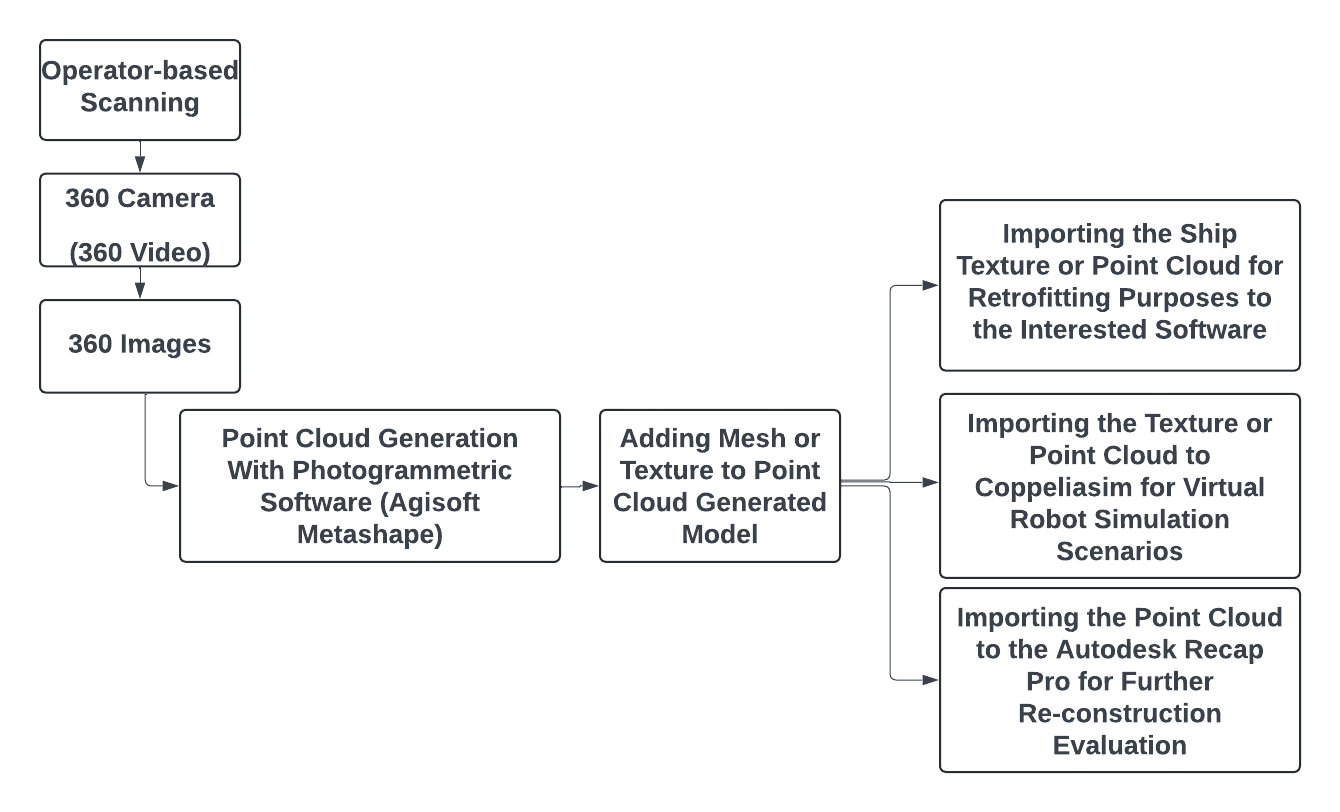
\includegraphics[width= 1.0\textwidth]{Figures/Project Flowchart.png}
  \caption[Illustration of Project Overview ]{Project Flowchart}
  \label{fig:Project Flowchart}
\end{figure}

In Figure \ref{fig:Project Flowchart}, I covered the project's overall outline, and the flow chart's square-shaped processes reflect sub-processes, which will be examined further in this chapter.


\subsection{Scanning with 360$^{\circ}$ Camera}
The first step that I need in this project is the scanning an asset or a scene to make a virtual point cloud of that object. Then I have my point could to make a 3D model. My industrial partner used QooCam 8K as you can see in Figure \ref{fig:QoooCam8K picture} for scanning the scene.  
\begin{figure}[H]
  \centering
  
\includegraphics[width= 1.0\textwidth]{Figures/QooCam8K.PNG}
  \caption[Picture of QooCam8K]{Picture of QooCam8K \cite{QooCam8K}}
  \label{fig:QoooCam8K picture}
\end{figure}
\noindent In the below Figure \ref{fig:QooCam8K Specification}, the specification of this 360 camera is shown:

\begin{figure}[H]
  \centering
  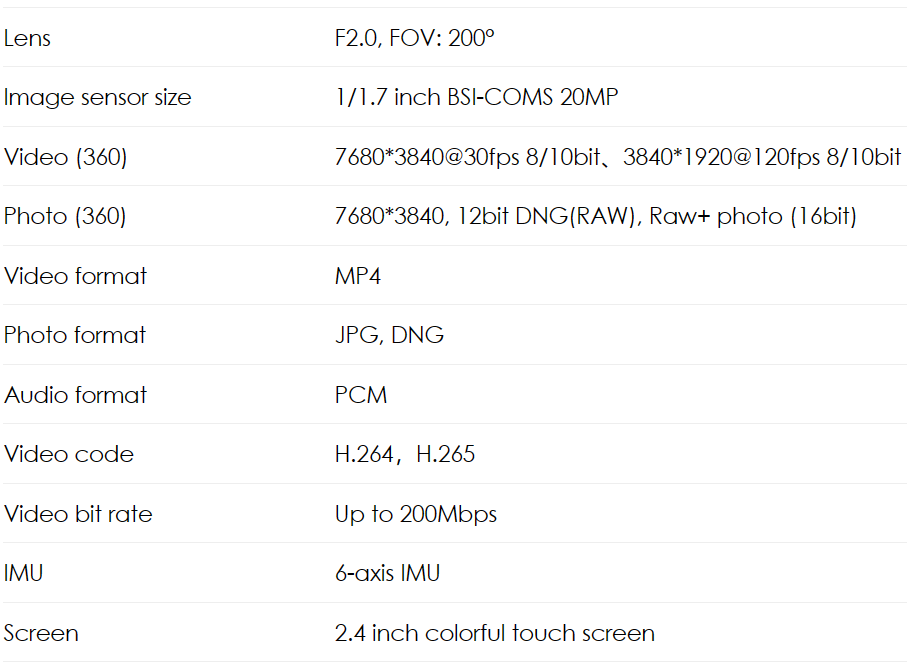
\includegraphics[width= 1.0\textwidth]{Figures/QooCam8KSPEC.PNG}
  \caption[Picture of QooCam8K Specification]{Picture of QooCam8K Specification \cite{QooCam8KSPEC}}
  \label{fig:QooCam8K Specification}
\end{figure}
 \textbf{Camera Features:} \\
I try to explain some features of this camera that is good to know for further work:
\begin{itemize}
    \item  \textbf{Lens F2.0}: F2.0 refers to the camera's aperture size. F2.0 permits more light to reach the image sensor. This can be useful in low-light settings without a flash. In general, the lower the F number, the more expensive the lens, and an F2.0 lens transports twice as much light as an f/4 lens. In Figure \ref{fig:Aperture Scale} aperture scale has been shown.  
\begin{figure}[H]
  \centering
  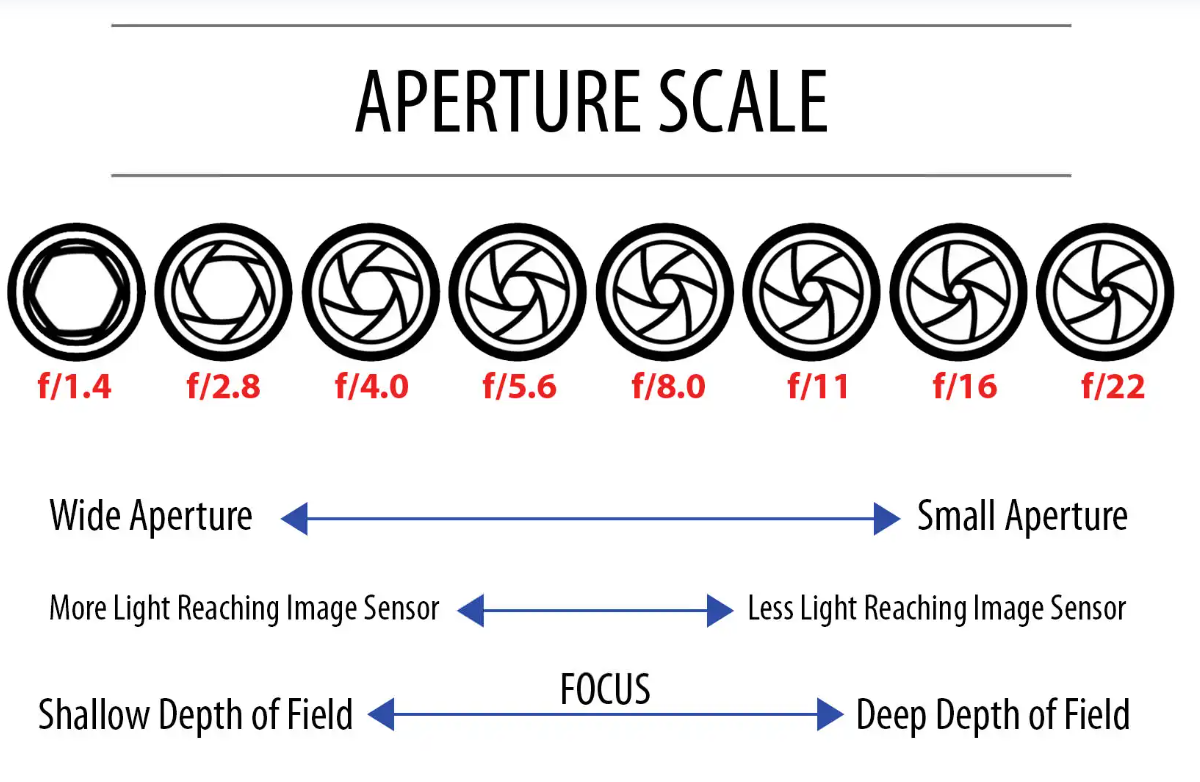
\includegraphics[width= 1.0\textwidth]{Figures/Aperture Scale.PNG}
  \caption[Picture of Aperture Scale]{Picture of Aperture Scale \cite{ApertureScale}}
  \label{fig:Aperture Scale}
\end{figure}
    
    The f-stop value indicates the amount of light entering the lens. Now comes the difficult part. Lower f-stop values allow more light to reach the lens. The greater the number, the less light. As a result, an aperture of f1.8 will let in far more light than an aperture of f2.2, resulting in superior, brighter photography in low-light situations such as night shots and some indoor photos. However, aperture affects more than just brightness. The depth of field is also directly related to the f-stop. A wider aperture, such as f1.8, produces a shallower depth of field, whilst a narrower aperture, such as f2.2, produces a deeper depth of field - so to extract the most detail from a shot, use the narrowest aperture \cite{lens}.


    \item  \textbf{FOV}: The field of view (FOV) is the open, viewable region that a person may see with their eyes or through an optical instrument like a camera. The maximum area that an optical instrument can capture is known as its field of view (FOV). FVO is related to two factors, the focal length of the lens and the sensor size. The focal length of a lens is the distance between the lens and the image being focused on the sensor. A bigger sensor provides a broader field of view at the same working distance. Changing the sensor size might alter the FOV. The sensor size is determined by the number and size of its pixels. Larger sensors produce a better image and have a higher resolution, whereas smaller sensors have a lower depth of field (DOF), resolution, and pixel size \cite{FOV,Fov}. In the Figure \ref{fig:Field of View of a Camera Lens} it shown the relation between field of view, focal length and sensor. 

 \begin{figure}[H]
  \centering
  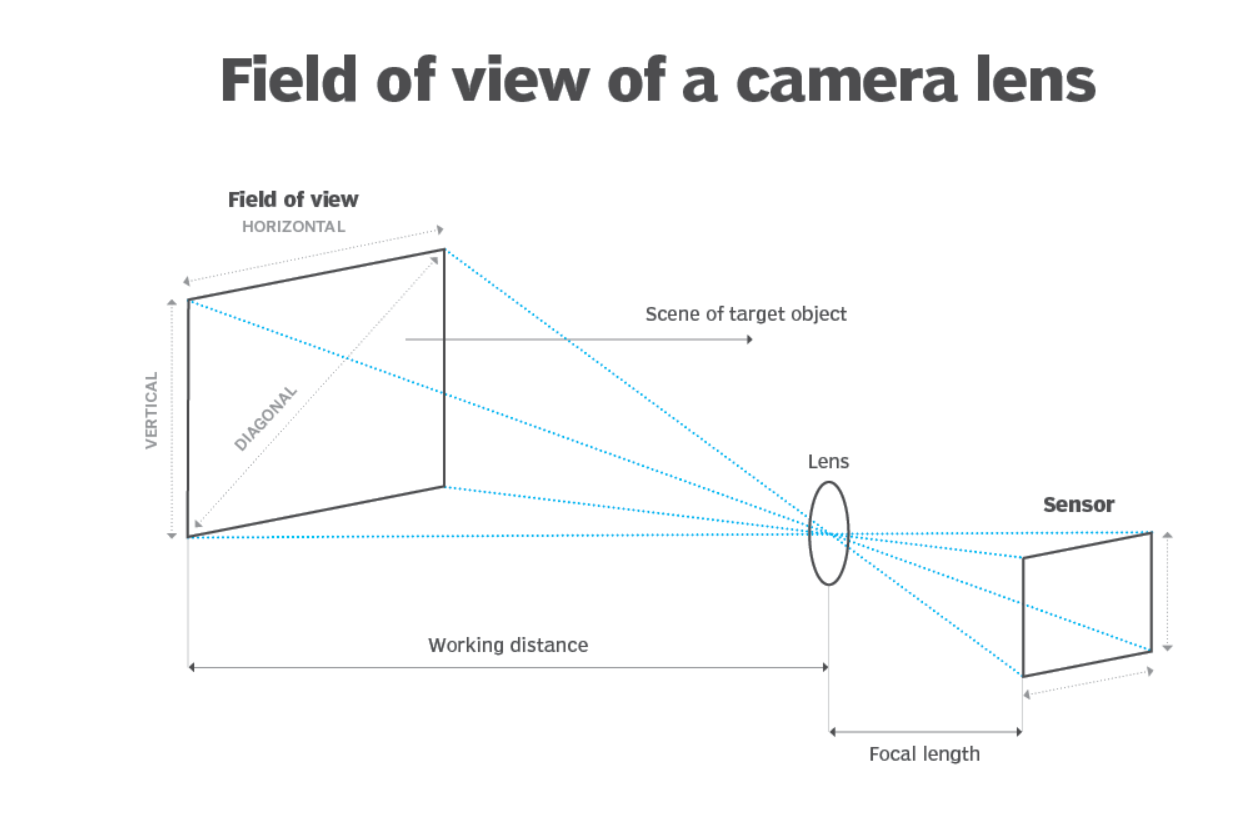
\includegraphics[width= 1.1\textwidth]{Figures/Field of View.PNG}
  \caption[Picture of Field of View of a Camera Lens]{Picture of Field of View of a Camera Lens \cite{FOV}}
  \label{fig:Field of View of a Camera Lens}
\end{figure}

    \item  \textbf{8K 30FPS or 4K 120FPS}:
QooCam8K is widely considered for 8K video recording with 30 frame per second or 4k with 120 frame per second.
In Figure \ref{fig:Different Resolution} the difference between the resolutions are visualized.
\begin{figure}[H]
  \centering
  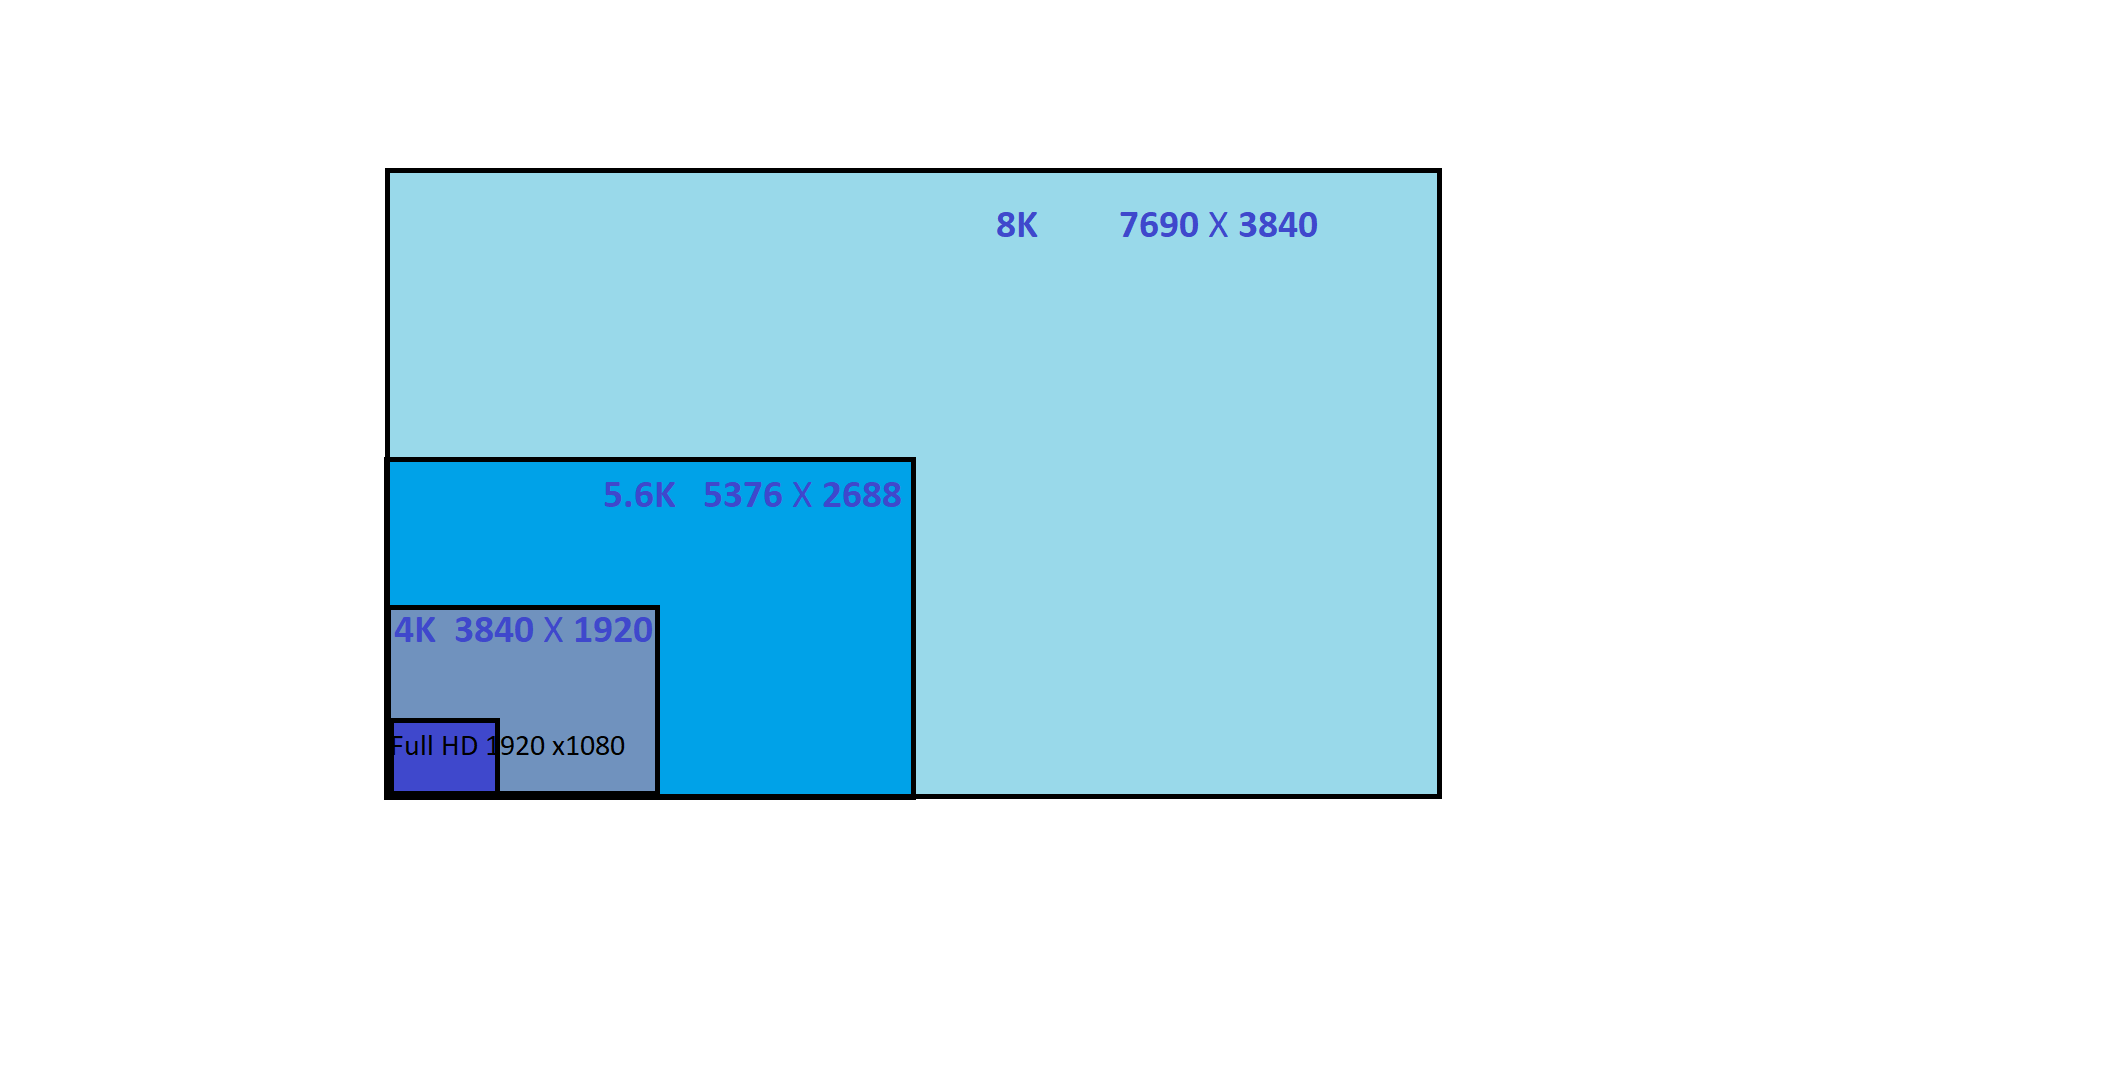
\includegraphics[width= 1.2\textwidth]{Figures/8K.PNG}
  \caption[Picture of Different resolutions]{Picture of Different Resolution}
  \label{fig:Different Resolution}
\end{figure}
 \noindent 4K 120FPS delivers the most cinematic 360 slow motion. Activities include skateboarding, paragliding, motocross, climbing, cycling, skiing, and surfing.Capture life's moments easily and turn them into spectacular slow motion.
    \item \textbf{10-Bit or 8-Bit Quality}:
    Color depth, also known as bit depth, is one of the parameters that define the quality of an image, whether still or video. They are the same thing. This is essentially a measure of how many shades and colors the camera can record; all other factors being equal, the more colors there are, the more complex and high-quality the footage can be. All photos captured by a digital camera contain red, green, and blue color information, and it is the combination of these color 'channels' that produces a full color image. So, when the camera is set to record in 8-bit video mode, it may capture footage with 256 levels for each color. This translates to a possibility of more than 16.7 million colors. If you set the quality to 10-bit video, you'll be capturing 1024 levels of color in each channel, with the potential for just over a billion different colors. However, it is worth noting that there is nothing wrong with 8-bit color. In fact, it is the style utilized in practically all of the videos you see on television or online.
 \cite{10Bit}. In Figure \ref{fig:Picture of Difference Betwwen 10-Bit and 8-Bit Video} the difference between 10-Bit and 8-Bit is more clear. 
\begin{figure}[H]
  \centering
  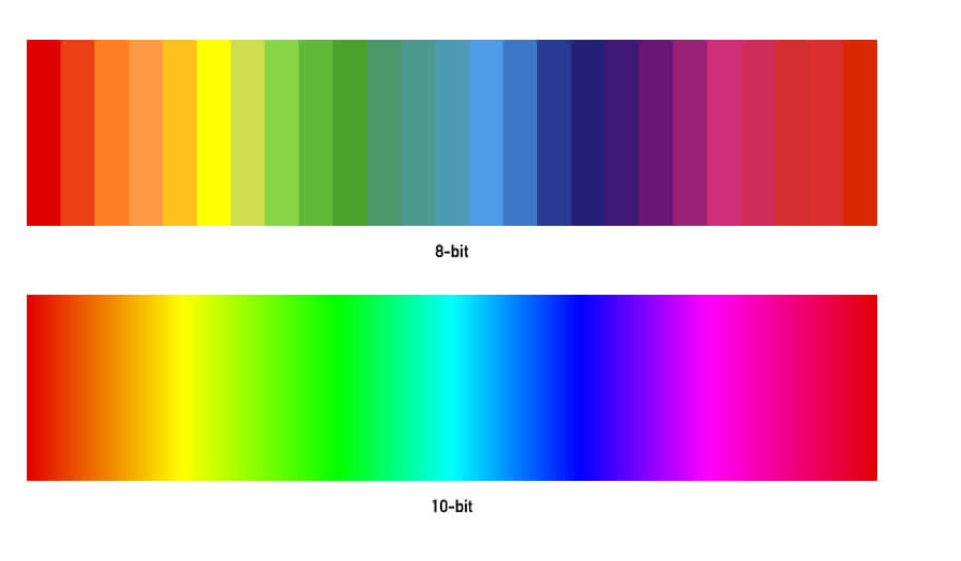
\includegraphics[width= 1.2\textwidth]{Figures/Bit.PNG}
  \caption[Picture of Difference Between 10-Bit and 8-Bit Video]{Picture of Difference Between 10-Bit and 8-Bit Video \cite{10Bit}}
  \label{fig:Picture of Difference Betwwen 10-Bit and 8-Bit Video}
\end{figure}
 
\end{itemize}
With QooCam8K scanned a hallway, in Figure \ref{fig:360 degree camera} the picture of hallway from 360 degree camera is shown.

\begin{figure}[H]
  \centering
  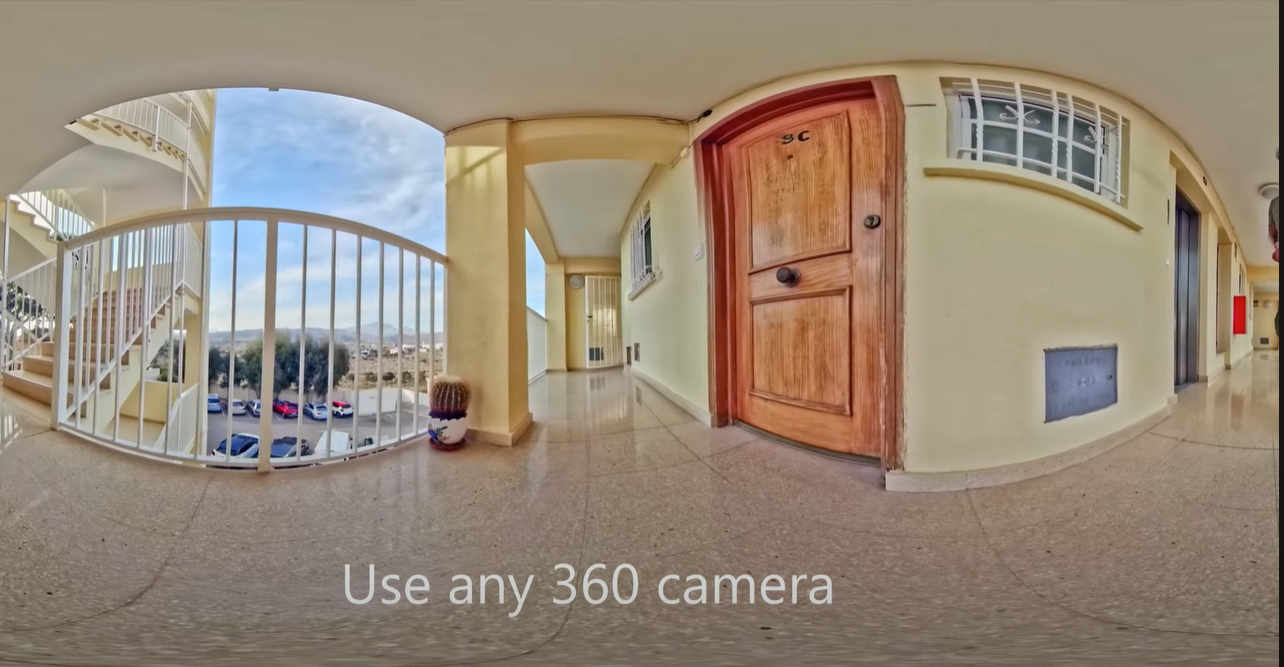
\includegraphics[width= 1.0\textwidth]{Figures/hallscan4.PNG}
  \caption[Picture of Hallway from 360 deegre camera]{Picture of hallway from 360 degree camera}
  \label{fig:360 degree camera}
\end{figure}
\noindent The hallway scan is made by ADAPA360 company as my industrial partner company. https://www.youtube.com/watch?v=5iUppdgs6TI \cite{ADAPA360}.\\

\noindent After scanning of the hallway with human-operator with low-speed  with 360 degree camera, then the scanned film imported to the Agisoft metashpe software for processing. This software make many frames of that footage, first aligned them and then stitch each image with neighbors images. Finally the point cloud is ready. It is also possible to visualize the point cloud in other software like Cloud Compare and Meshlab. In Figure \ref{fig:Camera Alignment in Agisoft} the camera alignment concept is visualized.  \\
\begin{figure}[H]
  \centering
  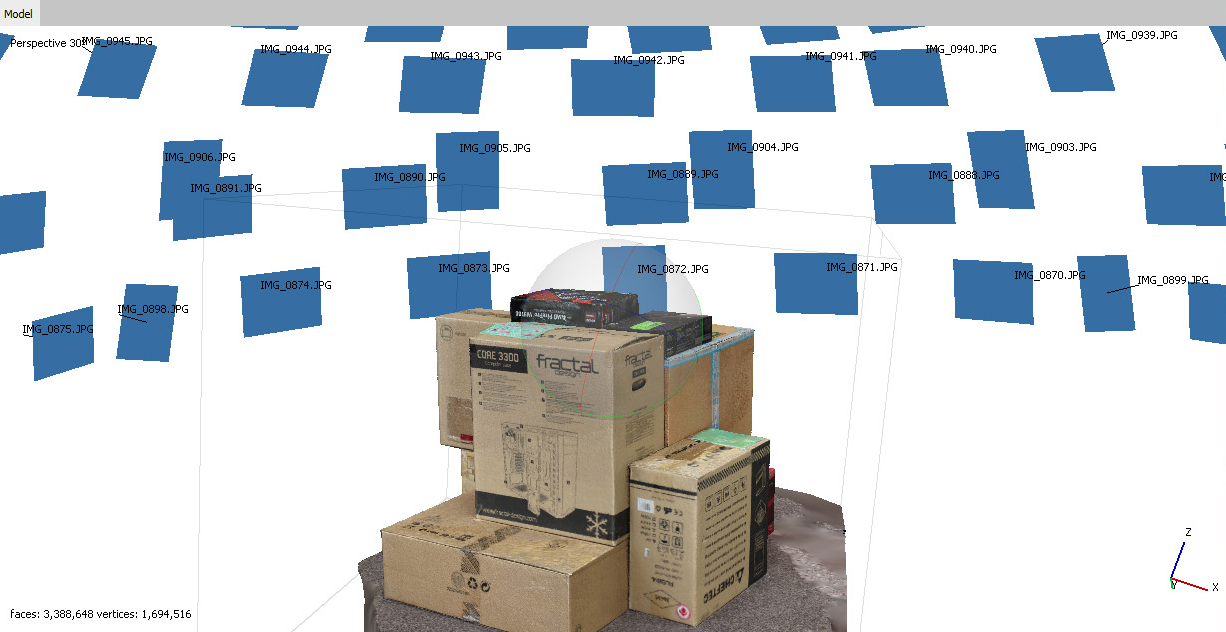
\includegraphics[width= 1.0\textwidth]{Figures/AgisoftCameraAlign.PNG}
  \caption[Camera Alignment in Agisoft]{Camera Alignment in Agisoft}
  \label{fig:Camera Alignment in Agisoft} \cite{Agisoft}
\end{figure}






 

%goal finding during avoiding the obstacles with different arrangement in the way. I used two algorithms 
\subsubsection{Concept for an UGV with Laser Scanner for Rescue Operations }
Imagine an autonomous ground robot just with laser scanner and without vision sensor wants to help for rescue operation in an unknown environment, what does it need to start the search. So, An autonomous robot developed for rescue operations must have several critical capabilities. \\

In the first step, it should be able to move around, overcome barriers, and adapt to diverse terrains. This allows the robot to reach regions that would otherwise be inaccessible or unsafe to humans. \\ 

Second, the robot should be equipped with a laser scanning sensor to detect its surroundings. This enables the robot to recognize and avoid obstacles while also locating targets, which is critical for effective rescue missions. \\

Third, the robot must have a communication mechanism to provide information back to the control center. This gives real-time updates on its location, status, and findings, allowing the control center to make educated decisions.\\

Fourth, the robot should have a dependable power source that allows it to function for long periods of time. This ensures that the robot can continue to operate without interruption.\\

Fifth, the robot should be resilient and robust enough to endure the extreme conditions common in disaster zones. This ensures the robot's durability and efficiency in these demanding conditions.\\

Sixth, the robot should have some degree of autonomy, allowing it to make decisions and complete tasks without continual human assistance. This boosts operational efficiency while reducing the workload on human operators.\\

If I want to summarize the robot operation into three main steps, there will be perception of surrounding environment by sensors and after that is decision making process based on the give algorithms and then actuation or movement until fulfilling the goal. 

\subsection{Algorithms for Making Decision }
I have used two types of implemented techniques for obstacle avoidance and motion planning purposes in CoppeliaSim. One technique is called potential field with gradient descent and another traditional technique is more robust for target finding low possibility of robot trapping and called vector field histogram plus(VFH+). 

\subsubsection{Motion Planning with Potential Fields }

In this part I introduce concepts in potential fields, main features and issues with this method.  There are two main forces for calculation in potential field, one is attractive force and another one is repulsive forces. Based on these two forces and calculations of gradient of the potential field, possible to control the robot \cite{Potentialfield}.    
\begin{itemize}
    \item  \textbf{ Potential function: }
\end{itemize}
 This is a scalar function and depends on the robot configuration \textit{q}, goal $q_{g}$, and obstacles $q_{o}$:\cite{khatib1986real} \\

\begin{equation}
\begin{aligned}
U(q, q_g, q_0) = U_{\text{attr}}(q, q_g) + U_{\text{rep}}(q, q_0)  
\end{aligned}
\label{eqn:potential function}
\end{equation} \\

\begin{figure}[h]
    \centering
    \begin{minipage}{0.45\textwidth}
        \centering
        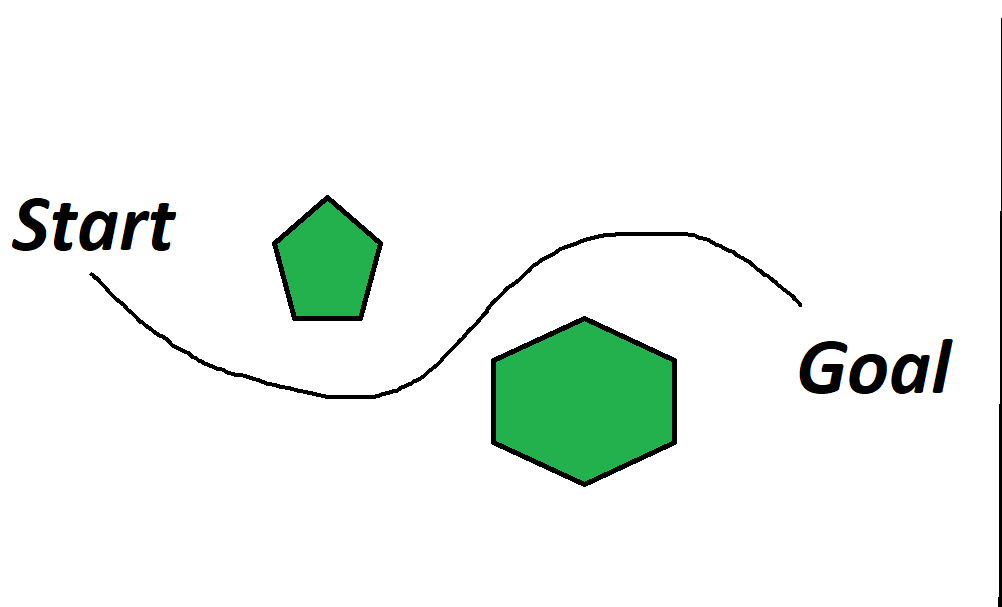
\includegraphics[width=0.9\textwidth]{Figures/graph.png} % first figure itself
        \caption{Start to Goal}
    \end{minipage}\hfill
    \begin{minipage}{0.45\textwidth}
        \centering
        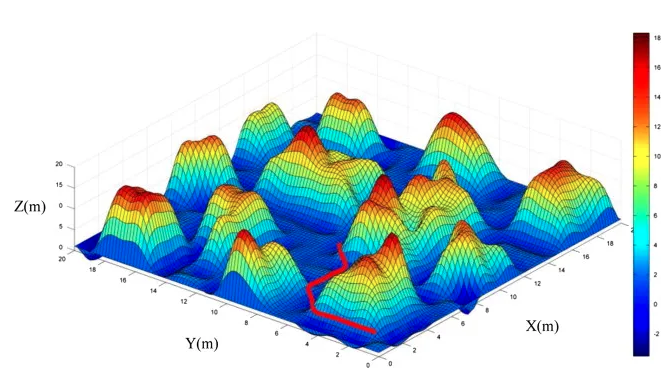
\includegraphics[width=0.9\textwidth]{Figures/graph2.PNG} % second figure itself
        \caption{Obstacles in 3D}
    \end{minipage}
\end{figure}

%------
\noindent \textbf {Attractive Potential Function}: This function depends on goal and robot configuration and based on this function the robots move towards the goal.
\\

\begin{itemize}
    \item  \textbf{ Quadratic Attractive Function (Parabolic): }\\
Quadratic function can take high values when the robot is far from the goal and the same is smooth in the vicinity og the goal.  
\begin{equation}
\begin{aligned}
U_{\text{attr}}(q, q_g) = \frac{1}{2} \epsilon_q d^2(q, q_g) \\
d(q, q_g) = \sqrt{(x - x_g)^2 + (y - y_g)^2}
\end{aligned}
\label{eqn:Quadratic Attractive Function}
\end{equation}  

     \item  \textbf{ Linear Attractive Function (Conic): }
The conic function is proportional to the distance between robot and the goal, however in the vicinity of the goal, the function will change abruptly.  
\begin{equation}
\begin{aligned}
U_{\text{attr}}(q, q_g) = \epsilon_c d(q, q_g)
\end{aligned}
\label{eqn: Linear Attractive Function}
\end{equation}  
\end{itemize}
\begin{figure}[h]
    \centering
    \begin{minipage}{0.45\textwidth}
        \centering
        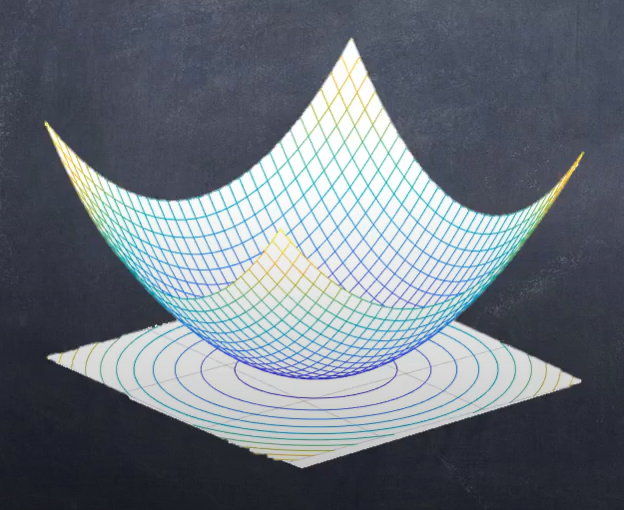
\includegraphics[width=0.9\textwidth]{Figures/Quad.PNG} % first figure itself
        \caption{Quadratic Function}
    \end{minipage}\hfill
    \begin{minipage}{0.45\textwidth}
        \centering
        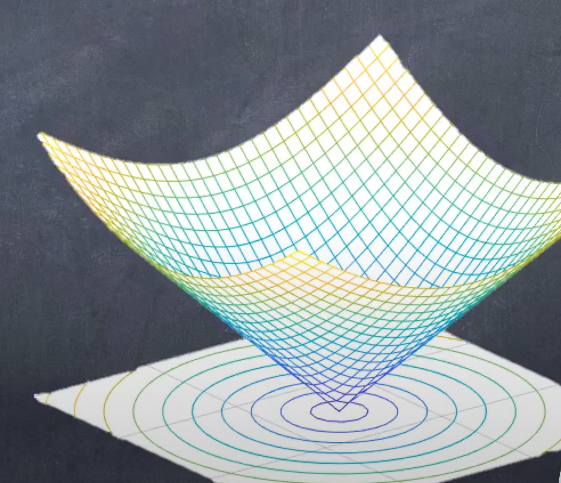
\includegraphics[width=0.9\textwidth]{Figures/Linear.PNG} % second figure itself
        \caption{Conic Function}
    \end{minipage}
\end{figure}

\begin{itemize}
      \item  \textbf{ Conic-parabolic Attractive Function: }
This function combines both conic and parabolic functions and define a distance threshold $Q_g$ and also a parabolic attractive constant. This function inside behaves parabolically which depends quadratically with the distance while from outside function behaves conically that it depends linearly with distance. 
\end{itemize}

\begin{equation}
\begin{aligned}
U_{\text{attr}}(q, q_g) = 
\begin{cases} 
\frac{1}{2} \epsilon_{q} d^2(q, q_g) & \text{if } d(q, q_g) < Q_g \\
Q_g \epsilon_{q} d(q,q_g) - \epsilon_{d} \frac{Q^2_g}{2} & \text{if } d(q, q_g) \geq Q_g 
\end{cases}
\end{aligned}
\label{eqn:Conic-parabolic attractive function}
\end{equation}  \\

\noindent \textbf {Repulsive Potential Function or Obstacle Avoidance Function}: This function parameters are dependent on the obstacle and robot configuration.This function avoids the robot from getting closer to the obstacles \cite{Pathplanning}.  

\begin{itemize}
      \item  \textbf{ Hyperbolic Repulsive Function: }
Repulsive function is defined by two distances, the first distance is beyond the specific distance that the robot has no influence on and the second distance is a minimum safety distance to avoid the obstacles, so if the robot has    
more distance than the threshold distance $Q_\text{inf}$ , the obstacles have no influence on it and if the robot is in area of the minimum distance $Q_\text{min}$ (safety distance) so the robot can not go closer to obstacle. And parameter $\epsilon_r$ modify how repulsive function effects to the robot. 
\end{itemize}

\begin{equation}
\begin{aligned}
U_{\text{rep}}(q, q_o) = 
\begin{cases} 
0 & \text{if } Q_{\text{inf}} \leq d(q, q_o), \\
\epsilon_r \left( \frac{1}{d(q, q_o)} - \frac{1}{Q_{\text{inf}}} \right) & \text{if } Q_{\text{min}} \leq d(q, q_o) \leq Q_{\text{inf}}, \\
\epsilon_r \left( \frac{1}{Q_{\text{min}}} - \frac{1}{Q_{\text{inf}}} \right) & \text{if } d(q, q_o) \leq Q_{\text{min}}.
\end{cases} 
\end{aligned}
\label{eqn: Hyperbolic Repulsive Function}
\end{equation}  \\

being $Q_{\text{min}}$ < $Q_{\text{inf}}$\\

\noindent \textbf {Total Potential Field}: This potential combines the attractive potential with the repulsive potential of obstacles, so the robot is attracted to a force field that pushes it towards the goal avoiding obstacles. 
\begin{equation}
\begin{aligned}
U(q, q_g, q_o) = U_{\text{attr}}(q, q_g) + \sum_i U_{\text{rep}}(q, q^{i}_o)
\end{aligned}
\label{eqn:Total Potential Field}
\end{equation} 
For the calculation of total potential function, I need distances to the goal and obstacle configuration and this can be done easily if a map is available but also considering sensor information. Total potential field can be used as state of control law with a known environment or as a sensor-based navigation method for global or local path-planning \cite{lu2014information}.  \\


\noindent \textbf {Gradient Descent}:
For planning a route,there is a need to follow the opposite direction of the gradient, because the gradient is a vector whose magnitude and direction will depend on the robot configuration, goal and obstacles. It is good to mention that locally the negative gradient will point in the direction that minimize the potential function (configuration with less energy),So the robot feels a force opposite to the gradient. \\
\begin{equation}
\begin{aligned}
\dot{q} = -\nabla U(q, q_g, q_o) = -\nabla U_{\text{attr}}(q, q_g) - \sum_i \nabla U_{\text{rep}}(q, q^{i}_o)
\end{aligned}
\label{eqn:Gradient Descent}
\end{equation} 

\noindent \textbf {Control Techniques}
\begin{itemize}
      \item  \textbf{ Force Control: }
To implement potential field technique, we need to compute the gradient of potential function, this gradient can be seen as a force that pushes the robot. In this case the effect of this force filtered by robot dynamic, so this type of control is generally smooth. And there would be some oscillations if the friction is not included in the dynamic of robot. 
\begin{equation}
\begin{aligned}
F = -\nabla U(q, q_g, q_o)
\end{aligned}
\label{eqn:Force Control}
\end{equation} 
      \item  \textbf{ Speed Control: }
Another typical alternative is to establish speed control so it means, here the speed is proportional to the gradient. The effect on the robot is independent of its dynamic which means robot is faster but it can produce sudden changes. In this case the most common implementation is the steepest descent method, it uses the unitary gradient vector and step size that the gradient step $lambda$ is a design parameter that can controls the amount of distance the robot can move \cite{LocalMinimum}.

\begin{equation}
\begin{aligned}
\dot{q} = -\nabla U(q, q_d, q_o) \\
q_{k+1} = q_k - \lambda \frac{\nabla U(q, q_d, q_o)}{\| \nabla U(q, q_d, q_o) \|}\\
\end{aligned}
\label{eqn:Speed Control}
\end{equation} 
\end{itemize}

\noindent \textbf {Local Minimum}\\
The attractive function has a single global minimum in the goal configuration; however, when combined with the repulsive function, local minimums may occur in some configurations that are difficult to predict if the entire configuration space is not well explored. This problem occurs where the gradient in the configuration becomes zero as a result of the balance of attracting and repulsive forces. Figure \ref{fig:Local Minimum} shows that there are some initial configurations from which the robot will not be able to reach the goal configuration. Local minimum are equilibrium points, so if we add some energy or little that might be enough to reach the goal configuration and the robot can escape from it. The type of this energy can be variant, there could be virtual forces, random movement, virtual objects or way-points.  

\begin{figure}[H]
  \centering
  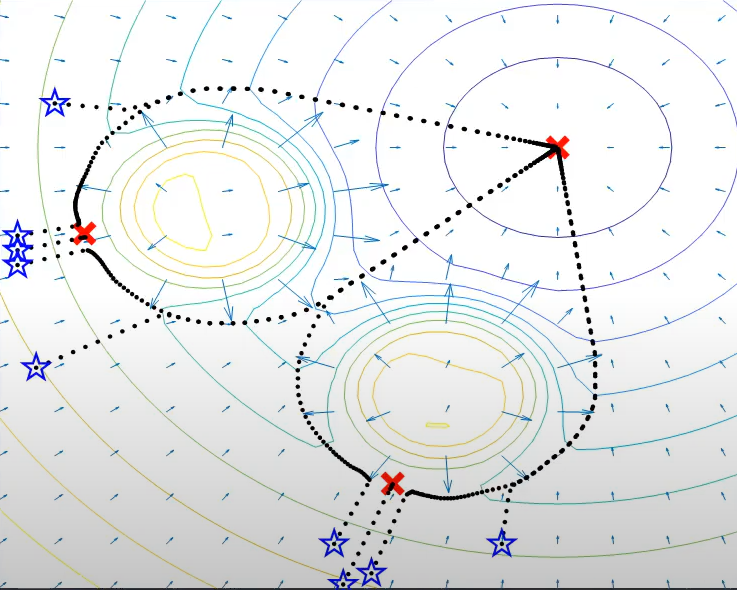
\includegraphics[width= 0.7\textwidth]{Figures/pot.PNG}
  \caption[Local Minimum]{Local Minimum} \cite{LocalMinimum}
   \label{fig:Local Minimum}
\end{figure}





\subsubsection{Motion Planning with Vector Fields Histogram plus (VFH+) an enhancement of VFH : }


  The vector field histogram (VFH) is a real-time obstacle avoidance system for mobile robotics. In VFH method there would be possible to make 2d occupancy map or cell histogram that enables for the incorporation of inaccurate measurements from sensors like ultrasound or laser and if 2d occupancy map or cell histogram is not available we can always use raw laser sensor data. In Figure \ref{fig:2d Occupancy Map} and Figure \ref{fig:cell histogram} sample of 2d occupancy map and cell histogram has been shown.
 

\begin{figure}[h]
    \centering
    \begin{minipage}{0.4\textwidth}
        \centering
        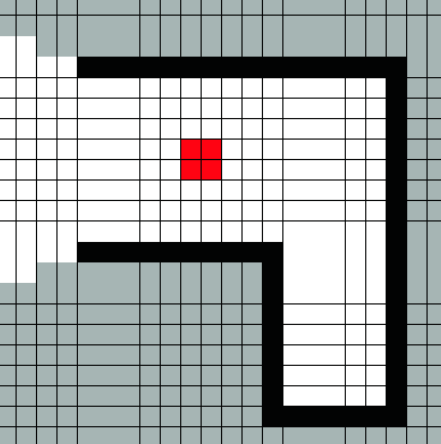
\includegraphics[width=0.9\textwidth]{Figures/2d Occupancy map.PNG} % first figure itself
        \caption{2d Occupancy Map \cite{Wang2018}}
        \label{fig:2d Occupancy Map}    
    \end{minipage}\hfill
    \begin{minipage}{0.5\textwidth}
        \centering
        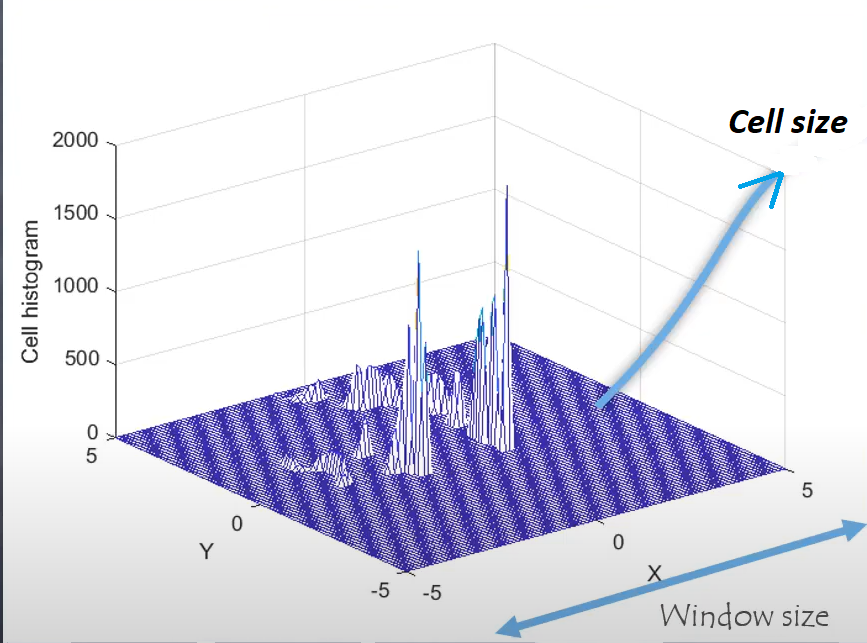
\includegraphics[width=0.9\textwidth]{Figures/cell histogram.PNG} 
        \caption{Cell Histogram \cite{Cellhistogram}} 
        \label{fig:cell histogram}
    \end{minipage}
\end{figure}

 \noindent The core concept of VFH method is to reduce this map to a polar histogram based on the preliminary ideas known as Virtual Field Force (VFF). Secondly valleys are detected in polar histogram to propose candidate directions to move and it means lower values of polar histogram in a given direction are less likely to face an obstacle. Also these valleys using threshold values and those sections that does not have threshold values means they are free sectors. When valleys have been detected are like set of sectors below the threshold and the one that is closest to the goal direction, will be selected and within that valley a direction according to the robot body size is selected to let the robot go forward. Now it should be distinguished that if it is wide or narrow valley\cite{VFH}. To understand how wide is a valley the VFH method improved to VFH+. VFH+ enhances the Vector Field Histogram (VFH) approach for real-time obstacle avoidance in mobile robots. The VFH+ approach improves robot trajectories and dependability. VFH+ simplifies parameter setting by accounting for robot width. VFH+ improves mobile robot trajectory accuracy, leading to increased reliability \cite{ulrich1998vfh+}. \\

   
 


\subsubsection{ Steps in VFH+ Method Implementation (Occupied Cells Detection and Obstacle Avoidance Method) }

Here I talked about all the VFH+ stages for data-reduction process that I need for computation of new direction toward goal with obstacle avoidance. \\

\textbf{ A. } First I need to make a cell histogram, whose values are updated based on the range sensor measurements.After several passes they will provide the certainty of the cells being occupied. Also I  can improve this stage by using occupancy maps which shows the likelihood of occupied cells. So the first stages of data reduction involves mapping the active region of the map grid to the principal polar histogram. The active region is a circular window (diameter Ws) that moves with the robot. The map grid treats each active cell's content as an obstacle vector. In the Figure \ref{fig:Histogram Grid Cells} shown an example of histogram grid cells and values. 
\begin{figure}[H]
  \centering
  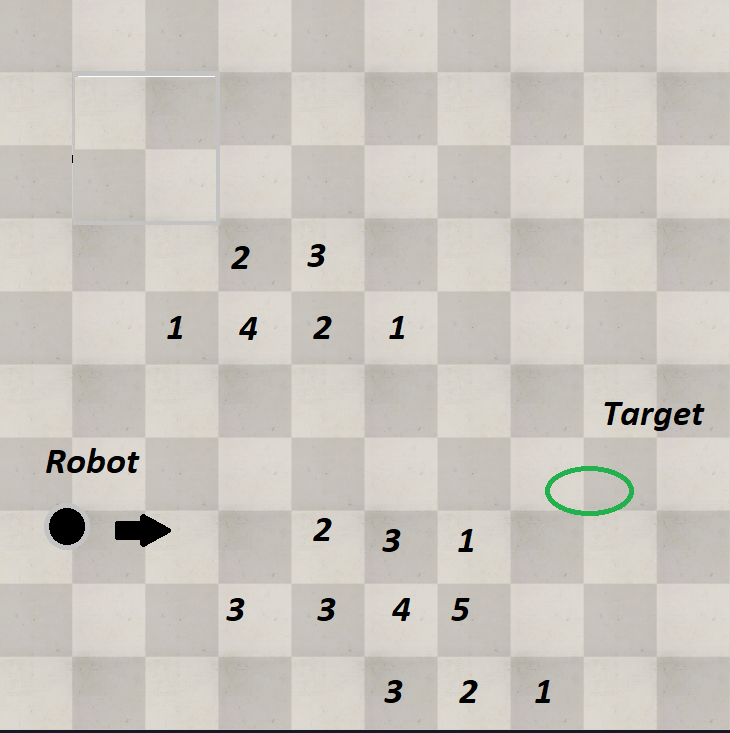
\includegraphics[width= 0.7\textwidth]{Figures/Grid.PNG}
  \caption[Histogram Grid Cells]{Histogram Grid Cells}
   \label{fig:Histogram Grid Cells} 
\end{figure}

\noindent \textbf{ B. } A 2d cell histogram will be converted to polar histogram that is a 1 dimensional histogram and in this process the size of the robot is taking into account.
For each cell a magnitude is computed depending on the cell distance to the robot and its occupancy likelihood and the magnitude are accumulated on their corresponding polar sector. In Figure \ref{fig:Active Cell's Magnitude and Assigned Sectors onto the Polar Histogram} a map of active cells on the polar histogram with each cell magnitude and the sectors have been shown. 
\begin{figure}[H]
  \centering
  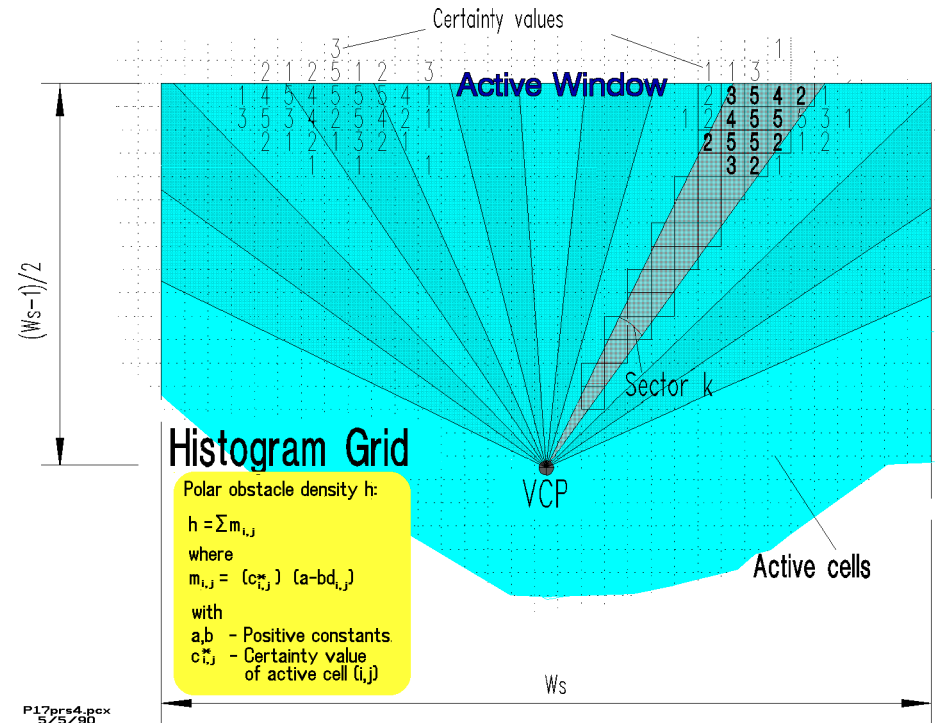
\includegraphics[width= 1.0\textwidth]{Figures/Active cells.PNG}
  \caption[Active Cell's Magnitude and Assigned Sectors onto the Polar Histogram]{Active Cell's Magnitude and Assigned Sectors onto the Polar Histogram}
   \label{fig:Active Cell's Magnitude and Assigned Sectors onto the Polar Histogram} \cite{Borenstein1991}
\end{figure}
\noindent Then it is possible to make 1d polar histogram with consideration of robot size as it is shown in Figure \ref{fig:Polar Histogram}. 
\begin{figure}[H]
  \centering
  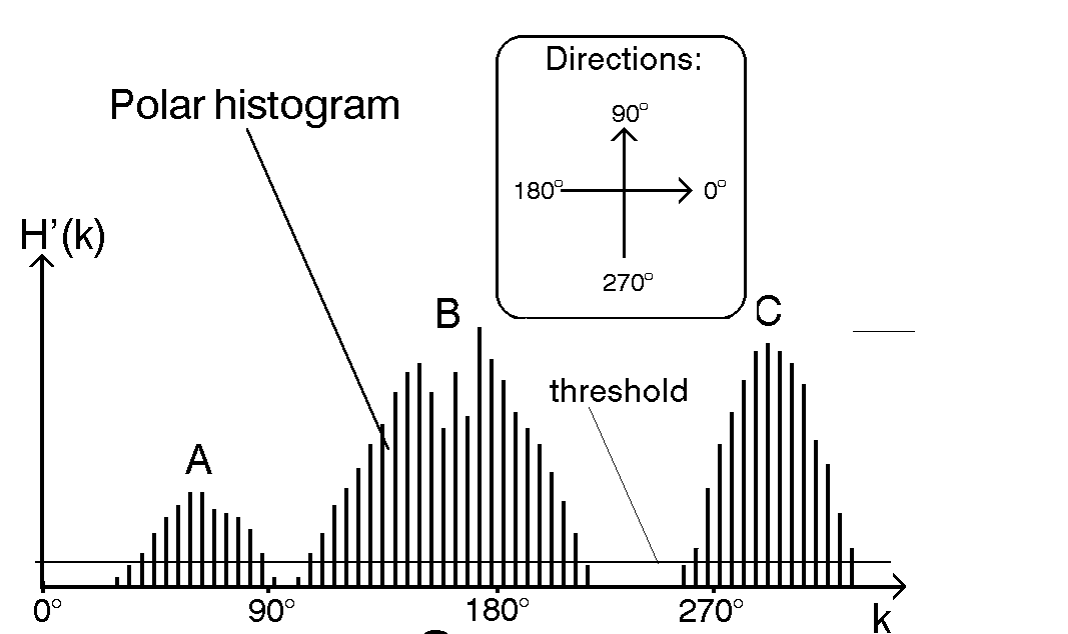
\includegraphics[width= 0.7\textwidth]{Figures/Polar Histogram.PNG}
  \caption[Polar Histogram]{Polar Histogram}
   \label{fig:Polar Histogram} \cite{Borenstein1991}
\end{figure}
\noindent \textbf{ C. } Next step is to making binary polar histogram to find the occupancy of sectors, for this purpose VFH+ method uses two thresholds to determine if a sector is occupied or free. If the value is more than the threshold the magnitude will be 1 and it means occupied and if the value is lower than the threshold the value is zero and means it is a free sector. If the values are between the thresholds ,the value of previous iteration will be used.  

\begin{equation}
\begin{aligned}
H_k^b = \begin{cases} 
1 & \text{if } H_k^p > \tau_{\text{high}} \\
0 & \text{if } H_k^p < \tau_{\text{low}} \\
H_k^p & \text{otherwise}
\end{cases}
\end{aligned}
\label{eqn:Speed Control}
\end{equation} 
In Figure \ref{fig:Binary Histogram} the binary histogram with thresholds is shown. 
\begin{figure}[H]
  \centering
  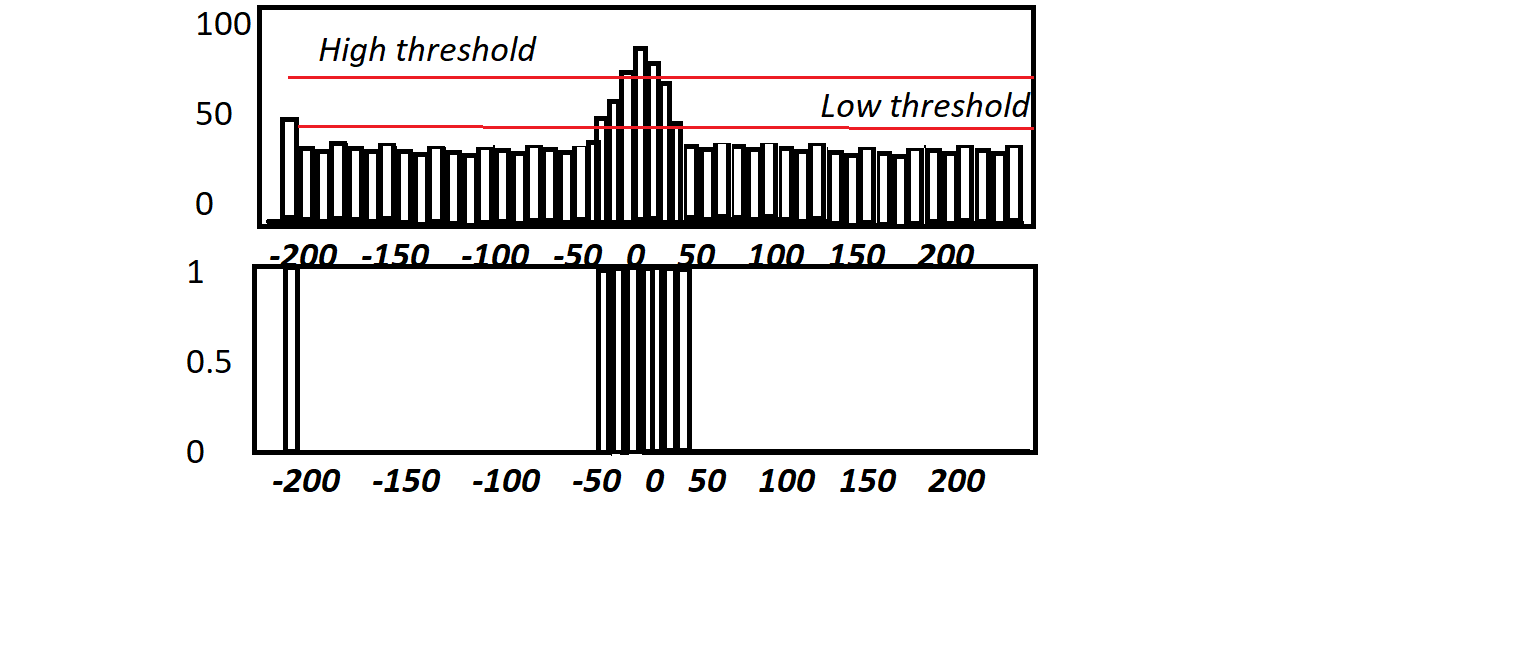
\includegraphics[width= 1.5\textwidth]{Figures/Binary histogram.png}
  \caption[Binary Histogram]{Binary Histogram}
   \label{fig:Binary Histogram} 
\end{figure}

\noindent \textbf{ D. }  The last histogram is the masked histogram, this histogram takes into account that the robot has some kinematic or dynamic constrains, therefore there is a minimum turning radius. This minimum turning radius imply that in-order to reach a free sector or sector that was categorized as a free in the binary histogram, I need to go through another sector that might be locked, then in that case those sectors will be also blocked. In Figure \ref{fig:2D Masked Histogram} and Figure \ref{fig:Binary and Masked Histogram}  visualized the the way that robot can decide between two obstacles by binary and masked histogram. As you can see the red zone in the masked histogram is marked as blocked direction because in order to reach those direction the robot must necessarily pass through the orange zone and due to minimum radius which is depicted in the blue circles in the  Figure \ref{fig:2D Masked Histogram}, this cannot be possible without colliding.   

\begin{figure}[H]
  \centering
  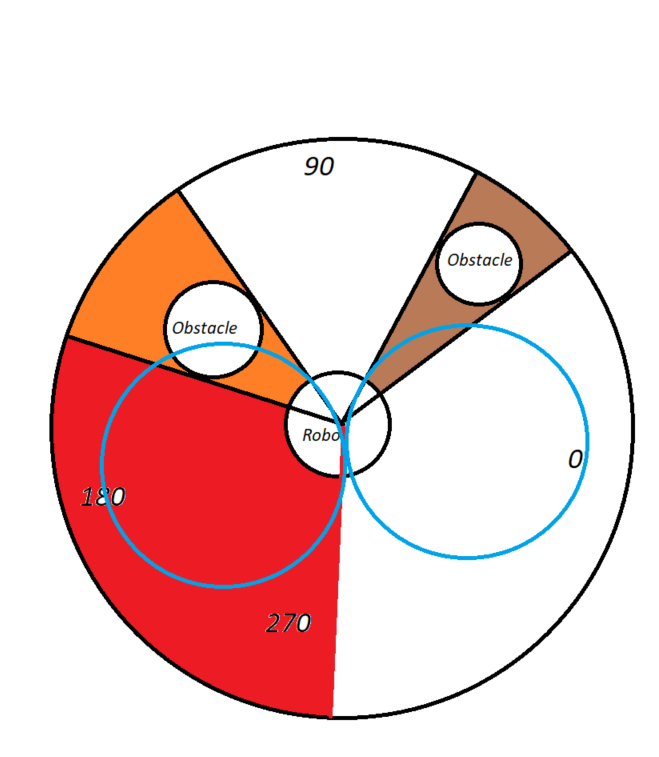
\includegraphics[width= 0.7\textwidth]{Figures/maskedcircle.PNG}
  \caption[2D Masked Histogram]{2D Masked Histogram}
   \label{fig:2D Masked Histogram} 
\end{figure}
\begin{figure}[H]
  \centering
  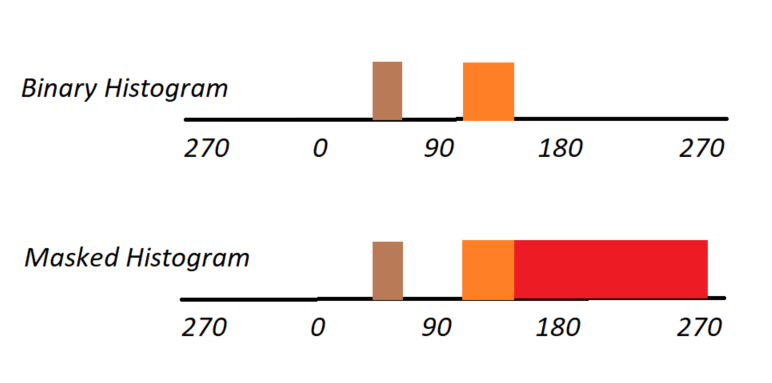
\includegraphics[width= 0.9\textwidth]{Figures/Binaryandmaskhis.PNG}
  \caption[Binary and Masked Histogram]{Binary and Masked Histogram}
   \label{fig:Binary and Masked Histogram} 
\end{figure}

\noindent \textbf{ E. } Once I have a masked histogram, then it is possible to detect the valleys which are set of sectors marked as free sectors. Two types of valleys are defined, narrow  and wide valleys. Narrow valley represent a region in which the robot can pass through but it is surrounded by obstacles, therefore this is only one possible direction which is just basically passed through the middle of the valley. A narrow valley shown in Figure \ref{fig:Narrow Valley in Histogram}. 

\begin{figure}[H]
  \centering
  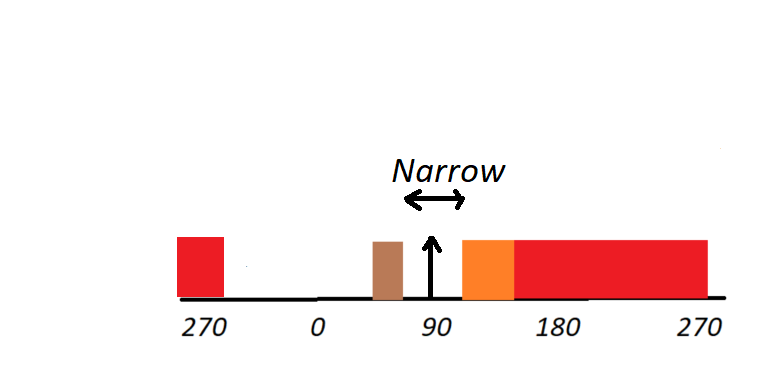
\includegraphics[width= 0.7\textwidth]{Figures/narrow.PNG}
  \caption[Narrow Valley in Histogram]{Narrow Valley in Histogram}
   \label{fig:Narrow Valley in Histogram} 
\end{figure}


\noindent On the other hand, there is wide valley which represents the region with obstacles far away from the robot, and in this case I usually can take three possible candidate directions to move through the left, the right edges or straight towards the goal if it is inside the valley. A wide valley shown in Figure \ref{fig:Wide Valley in Histogram}. 
\begin{figure}[H]
  \centering
  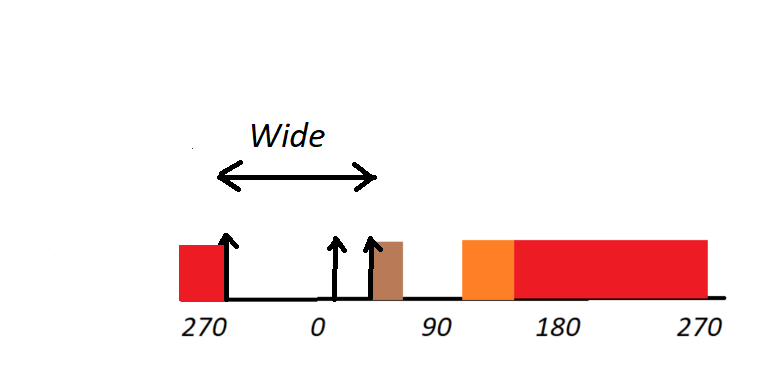
\includegraphics[width= 0.7\textwidth]{Figures/wide.PNG}
  \caption[Wide Valley in Histogram]{Wide Valley in Histogram}
   \label{fig:Wide Valley in Histogram} 
\end{figure}


\noindent Now among all possible directions,I need to select the best route and for this purpose the VFH+ algorithm define a cost function that I need to minimize it by considering tree terms such as target weight $W_t \Delta(c,t)$, previous direction weight $W_p \Delta( c ,p)$ and current robot's direction weight $W_c \Delta (c)$ . The ways of these three criteria allow us to implement different behaviors in the algorithm. In equation \eqref{eqn:Cost Function}
the cost function based on these three criteria is written. 
\begin{equation}
\begin{aligned}
f(c) = W_t \Delta(c,t) + W_p \Delta ( c , p) + W_c \Delta (c)
\end{aligned}
\label{eqn:Cost Function}
\end{equation} 
The first term of cost function $W_t$, indicates the cost associated with the difference between the candidate and target directions. The larger the disparity, the expense of guiding the robot away from its desired direction increases as the number of candidate directions increase \cite{Borenstein1991}.\\
The third term $W_p$ calculates the cost of moving in a different direction compared to the previously chosen one. The higher the difference, the greater the effect of the new steering command\cite{Borenstein1991}.\\
The second term $W_c$ calculates the cost of the difference between a candidate direction and the robot's current wheel alignment. The greater the disparity, the greater the need to shift direction of travel\cite{Borenstein1991}.\\


